\chapter{Directed graphical models (Bayes nets)}


\section{Introduction}


\subsection{Chain rule}
\begin{equation}
p(x_{1:V}) = p(x_1)p(x_2|x_1)p(x_3|x_{1:2})\cdots p(x_N|x_{1:V-1})
\end{equation}

\subsection{Conditional independence}
$X$ and $Y$ are \textbf{conditionally independent} given $Z$, denoted $X \perp Y|Z$, iff the conditional joint can be written as a product of conditional marginals, i.e.
\begin{equation}
X \perp Y|Z \Longleftrightarrow p(X,Y|Z)=p(X|Z)p(Y|Z)
\end{equation}

first order \textbf{Markov assumption}: the future is independent of the past given the present, 
\begin{equation}
x_{t+1} \perp x_{1:t-1}|x_t
\end{equation}

first-order \textbf{Markov chain}
\begin{equation}
p(x_{1:V}) = p(x_1)\prod\limits_{t=2}^V p(x_t|x_{t-1})
\end{equation}


\subsection{Graphical models}
A \textbf{graphical model}(GM) is a way to represent a joint distribution by making CI assumptions. In particular, the nodes in the graph represent random variables, and the (lack of) edges represent CI assumptions.

There are several kinds of graphical model, depending on whether the graph is directed, undirected, or some combination of directed and undirected. In this chapter, we just study directed graphs. We consider undirected graphs in Chapter 19.


\subsection{Directed graphical model}
A \textbf{directed graphical model}or \textbf{DGM} is a GM whose graph is a DAG. These are more commonly known as \textbf{Bayesian networks}. However, there is nothing inherently “Bayesian” about Bayesian networks: they are just a way of defining probability distributions. These models are also called \textbf{belief networks}. The term “belief” here refers to subjective probability. Once again, there is nothing inherently subjective about the kinds of probability distributions represented by DGMs.

\textbf{Ordered Markov property}
\begin{equation}
x_s \perp x_{\mathrm{pred}(s)\ \mathrm{pa}(s)} \perp x_{\mathrm{pa}(s)}
\end{equation}
where pa$(s)$ are the parents of nodes, and pred$(s)$ are the predecessors of nodes in the DAG.

\textbf{\textbf{Markov chain}} on a DGM
\begin{equation}
p(x_{1:V}|G)=\prod\limits_{t=1}^V p(x_t|x_{\mathrm{pa}(t)})
\end{equation}


\begin{figure}[hbtp]
\centering
    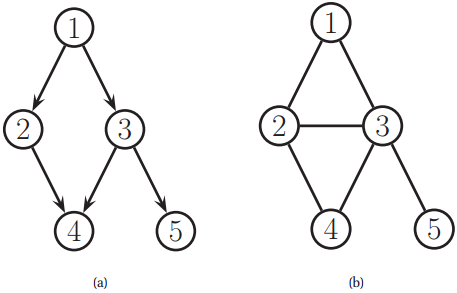
\includegraphics[scale=.70]{graphical-models.png}
\caption{(a) A simple DAG on 5 nodes, numbered in topological order. Node 1 is the root, nodes 4 and 5 are the leaves. (b) A simple undirected graph, with the following maximal cliques: {1,2,3}, {2,3,4}, {3,5}.}
\label{fig:graphical-models} 
\end{figure}


\section{Examples}


\subsection{Naive Bayes classifiers}
\begin{figure}[hbtp]
\centering
    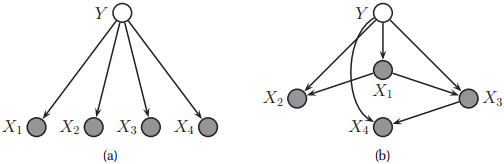
\includegraphics[scale=.70]{naive-bayes-as-DGM.png}
\caption{(a) A naive Bayes classifier represented as a DGM. We assume there are $D=4$ features, for simplicity. Shaded nodes are observed, unshaded nodes are hidden. (b) Tree-augmented naive Bayes classifier for $D=4$ features. In general, the tree topology can change depending on the value of $y$.}
\label{fig:naive-bayes-as-DGM} 
\end{figure}


\subsection{Markov and hidden Markov models}
\begin{figure}[hbtp]
\centering
    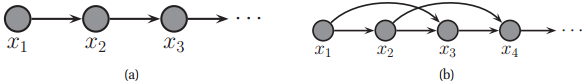
\includegraphics[scale=.70]{second-order-Markov-chain.png}
\caption{A first and second order Markov chain.}
\label{fig:second-order-Markov-chain} 
\end{figure}

\begin{figure}[hbtp]
\centering
    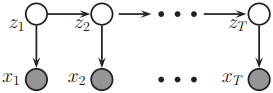
\includegraphics[scale=.70]{first-order-HMM.png}
\caption{A first-order HMM.}
\label{fig:first-order-HMM} 
\end{figure}



\section{Inference}
Suppose we have a set of correlated random variables with joint distribution $p(\vec{x}_{1:V}|\vec{\theta})$. Let us partition this vector into the \textbf{visible variables} $\vec{x}_v$, which are observed, and the \textbf{hidden variables}, $\vec{x}_h$, which are unobserved. Inference refers to computing the posterior distribution of the unknowns given the knowns:
\begin{equation}
p(\vec{x}_h|\vec{x}_v,\theta) = \frac{p(\vec{x}_h, \vec{x}_v|\vec{\theta})}{p(\vec{x}_v|\vec{\theta})}=\frac{p(\vec{x}_h, \vec{x}_v|\vec{\theta})}{\sum_{\vec{x}_h'}p(\vec{x}_h', \vec{x}_v|\vec{\theta})}
\end{equation}

Sometimes only some of the hidden variables are of interest to us. So let us partition the hidden variables into \textbf{query variables}, $\vec{x}_q$, whose value we wish to know, and the remaining \textbf{nuisance variables}, $\vec{x}_n$, which we are not interested in. We can compute what we are interested in by \textbf{marginalizing out} the nuisance variables:
\begin{equation}
p(\vec{x}_q|\vec{x}_v,\vec{\theta}) = \sum_{\vec{x}_n}p(\vec{x}_q, \vec{x}_n|\vec{x}_v, \vec{\theta})
\end{equation}


\section{Learning}
MAP estimate:
\begin{equation}
\hat{\vec{\theta}} =\arg\max_{\vec{\theta}}\sum\limits_{i=1}^N \log p(\vec{x}_{i,v}|\vec{\theta})+\log p(\vec{\theta})
\end{equation}


\subsection{Learning from complete data}
If all the variables are fully observed in each case, so there is no missing data and there are no hidden variables, we say the data is \textbf{complete}. For a DGM with complete data, the likelihood is given by
\begin{equation}
p(\mathcal{D}|\vec{\theta}) = \prod_{i=1}^N p(\vec{x}_i|\vec{\theta})
= \prod_{i=1}^N\prod_{t=1}^V p(\vec{x}_{it}|\vec{x}_{i, \mathrm{pa}(t)}, \vec{\theta}_t)
= \prod_{t=1}^V p(\mathcal{D}_t|\vec{\theta}_t)
\end{equation}
where $\mathcal{D}_t$ is the data associated with node $t$ and its parents, i.e., the $t$'th family.

Now suppose that the prior factorizes as well:
\begin{equation}
p(\vec{\theta})=\prod\limits_{t=1}^V p(\vec{\theta}_t)
\end{equation}

Then clearly the posterior also factorizes:
\begin{equation}
p(\vec{\theta}|\mathcal{D}) \propto p(\mathcal{D}|\vec{\theta})p(\vec{\theta}) = \prod\limits_{t=1}^V p(\mathcal{D}_t|\vec{\theta}_t)p(\vec{\theta}_t)
\end{equation}


\subsection{Learning with missing and/or latent variables}
If we have missing data and/or hidden variables, the likelihood no longer factorizes, and indeed it is no longer convex, as we explain in detail in Section TODO. This means we will usually can only compute a locally optimal ML or MAP estimate. Bayesian inference of the parameters is even harder. We discuss suitable approximate inference techniques in later chapters.


\section{Conditional independence properties of DGMs}


\subsection{d-separation and the Bayes Ball algorithm (global Markov properties)}
\begin{enumerate}
\item P contains a chain
\begin{equation}
p(x,z|y) = \frac{p(x,y,z)}{p(y)}
= \frac{p(x)p(y|x)p(z|y)}{p(y)}
= \frac{p(x,y)p(z|y)}{p(y)} = p(x|y)p(z|y)
\end{equation}

\item P contains a fork
\begin{equation}
p(x,z|y) = \frac{p(x,y,z)}{p(y)}
= \frac{p(y)p(x|y)p(z|y)}{p(y)}
= p(x|y)p(z|y)
\end{equation}
\item P contains v-structure
\begin{equation}
p(x,z|y) = \frac{p(x,y,z)}{p(y)}
= \frac{p(x)p(z)p(y|x,z)}{p(y)}
\neq p(x|y)p(z|y)
\end{equation}
\end{enumerate}



\subsection{Other Markov properties of DGMs}


\subsection{Markov blanket and full conditionals}

\begin{equation}
mb(t) = ch(t)\cup pa(t)\cup copa(t)
\end{equation}


\subsection{Multinoulli Learning}
Multinoulli Distribution:
\begin{equation}
Cat(x|\mu) = \prod_{k=1}^K\mu_k^{x_k}
\label{discrite}
\end{equation}
then from \ref{bayes_net} and \ref{discrite}:
\begin{equation}
p(x|G,\theta) = \prod_{v=1}^V\prod_{c=1}^{C_v}\prod_{k=1}^K
\theta_{vck}^{y_{vck}}
\end{equation}
Likelihood
\begin{equation}
p(D|G,\theta) = \prod_{n=1}^N p(x_n|G,\theta)
=\prod_{n=1}^N\prod_{v=1}^V\prod_{c=1}^{C_{nv}}\prod_{k=1}^K
\theta_{vck}^{y_{nvck}}
\end{equation}
where $y_{nv} = f(pa(x_{nv}))$, f(x) is a map from x to a vector,
there is only one element in the vector is 1.


\section{Influence (decision) diagrams *}

